\section{Relation and Digraphs}
\subsection{Introduction to binary relations}

A \textbf{Binary Relation} between two sets $A$ and $B$ is a subset $R$ of $A \times B$.
It is binary because it is between two sets.
\[
  \text{for } a \in A \land b \in B, (a,b) \in R \text{ is denoted as } a\text{R}b
\]

For example, consider the relation C between $\mathbb{R}$ and $\mathbb{Z}$:
\[
  x\text{C}y \text{ if } \left\lvert x-y\right\rvert \leq 1, \text{ where } x \in \mathbb{R} \text{ and } y \in \mathbb{Z}
\]
If $A$ and $B$ are finite, then relation R between $A$ and $B$ can be represented by a set of ordered pairs.

\subsubsection*{Matrix Representation}
\begin{align*}
  P           & = \{\text{Sue}, \text{Harry}, \text{Sam}\}                       \\
  \text{File} & = \{\text{File A}, \text{File B}, \text{File C}, \text{File D}\}
\end{align*}
\[
  \bordermatrix{ & \text{File A} & \text{File B} & \text{File C} & \text{File D} \cr
    \text{Sue}   & 0 & 1 & 1 & 1 \cr
    \text{Harry} & 1 & 0 & 0 & 0 \cr
    \text{Sam}   & 0 & 0 & 0 & 0 \cr }
\]
\begin{center}
  An element is
  \begin{tabular}{c}
    1 if $p$R$f$ is true \\
    0 if $p$R$f$ is false
  \end{tabular}
\end{center}

\subsubsection*{Arrow Diagram}
\begin{align*}
  A & = \{a,b,c,d,e\}                                \\
  R & \subseteq A \times A                           \\
  R & = \{(a,b), (b,c), (e,c), (c,e), (d,a), (d,d)\}
\end{align*}
\begin{center}
  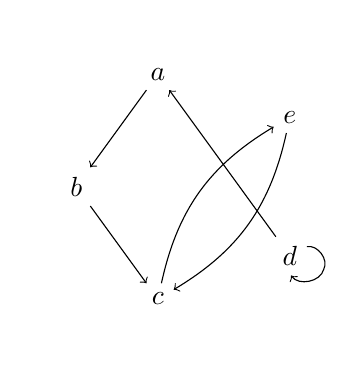
\begin{tikzpicture}
    %VARIABLES
    \pgfmathsetmacro{\gsize}{1.5}
    \pgfmathsetmacro{\gnum}{5}

    \foreach[count=\i] \element in {a,b,c,d,e} { %domain
        \node (\element) at (\i * 360 / \gnum + 180 / \gnum:\gsize) {$\element$};
        \node (\element-) at (\i * 360 / \gnum + 180 / \gnum:\gsize + 0.5) {};
      }
    \foreach \j/\l in {a/b,b/c,d/a} { %a to b
        \draw[->] (\j) -- (\l);
      }
    \foreach \j/\l in {e/c} { %a to b AND b to a
        \draw[->] (\j) to[bend left=20 / \gsize + 10] (\l);
        \draw[->] (\l) to[bend left=20 / \gsize + 10] (\j);
      }
    \foreach \j in {d} { %a to a
        \draw[->] (\j) to[bend left=65] (\j-)
        to[bend left=65] (\j);
      }
  \end{tikzpicture}
\end{center}

\subsubsection*{Arrow Diagram vs. Matrix Representation}
\begin{align*}
  A & = \{1,2,3,4\}                                  \\
  R & = \{(1,2), (1,3), (2,2), (2,3), (3,4), (4,3)\}
\end{align*}
\begin{center}
  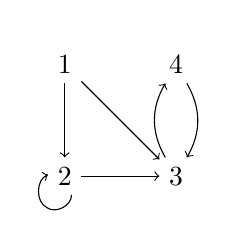
\begin{tikzpicture}
    %VARIABLES
    \pgfmathsetmacro{\gsize}{1}
    \pgfmathsetmacro{\gnum}{4}

    \foreach[count=\i] \element in {1,2,3,4} { %domain
        \node (\element) at (\i * 360 / \gnum + 180 / \gnum:\gsize) {$\element$};
        \node (\element-) at (\i * 360 / \gnum + 180 / \gnum:\gsize + 0.5) {};
      }
    \foreach \j/\l in {1/2,1/3,2/3} { %a to b
        \draw[->] (\j) -- (\l);
      }
    \foreach \j/\l in {3/4} { %a to b AND b to a
        \draw[->] (\j) to[bend left=20 / \gsize + 10] (\l);
        \draw[->] (\l) to[bend left=20 / \gsize + 10] (\j);
      }
    \foreach \j in {2} { %a to a
        \draw[->] (\j) to[bend left=65] (\j-)
        to[bend left=65] (\j);
      }
  \end{tikzpicture}
  \qquad
  $
    \bordermatrix{ & 1 & 2 & 3 & 4 \cr
      1 & 0 & 1 & 1 & 0 \cr
      2 & 0 & 1 & 1 & 0 \cr
      3 & 0 & 0 & 0 & 1 \cr
      4 & 0 & 0 & 1 & 0 \cr }
  $
\end{center}

\subsection{Properties of binary relations}

A binary relation of R on set $A$ is \textbf{Reflective} if for \textit{every} $x \in A$, $x$R$x$.
For Arrow Diagrams, this means the graph contains self-loops:
\begin{center}
  \begin{tikzpicture}
    %VARIABLES
    \pgfmathsetmacro{\gsize}{1}
    \pgfmathsetmacro{\gnum}{2}

    \foreach[count=\i] \element in {a,b} { %domain
        \node (\element) at (\i * 360 / \gnum:\gsize) {$\element$};
        \node (\element-) at (\i * 360 / \gnum:\gsize + 0.5) {};
      }
    \foreach \j in {a,b} { %a to a
        \draw[->] (\j) to[bend left=65] (\j-)
        to[bend left=65] (\j);
      }
  \end{tikzpicture}
\end{center}
For Matrix Representation, this means that the top left to bottom right diagonal are all 1's:
\[
  \bordermatrix{ & a & b & c & d \cr
    a & 1 & - & - & - \cr
    b & - & 1 & - & - \cr
    c & - & - & 1 & - \cr
    d & - & - & - & 1 \cr }
\]

A binary relation of R on set $A$ is \textbf{Anti-reflective} if for \textit{every} $x \in A$, $x$R$x$ is \textit{not} true.
For Arrow Diagrams, this means the graph does not contain self-loops:
\begin{center}
  \begin{tikzpicture}
    %VARIABLES
    \pgfmathsetmacro{\gsize}{1}
    \pgfmathsetmacro{\gnum}{2}

    \foreach[count=\i] \element in {a,b} { %domain
        \node (\element) at (\i * 360 / \gnum:\gsize) {$\element$};
        \node (\element-) at (\i * 360 / \gnum:\gsize + 0.5) {};
      }
  \end{tikzpicture}
\end{center}
For Matrix Representation, this means that the top left to bottom right diagonal are all 0's:
\[
  \bordermatrix{ & a & b & c & d \cr
    a & 0 & - & - & - \cr
    b & - & 0 & - & - \cr
    c & - & - & 0 & - \cr
    d & - & - & - & 0 \cr }
\]

A binary relation of R on set $A$ is \textbf{Symmetric} if and only if for \textit{every} pair $x \in A$, $y \in Y$,
either \textit{both} $x$R$y$ \underline{and} $y$R$x$, or \textit{both} not $x$R$y$ or not $y$R$x$ is true.
For Arrow Diagrams, this means that every arrow has an arrow going the other way:
\begin{center}
  \begin{tikzpicture}
    %VARIABLES
    \pgfmathsetmacro{\gsize}{1}
    \pgfmathsetmacro{\gnum}{4}

    \foreach[count=\i] \element in {a,b,c} { %domain
        \node (\element) at (\i * 360 / \gnum:\gsize) {$\element$};
        \node (\element-) at (\i * 360 / \gnum:\gsize + 0.5) {};
      }
    \foreach \j/\l in {a/b,b/c} { %a to b AND b to a
        \draw[->] (\j) to[bend left=20 / \gsize + 10] (\l);
        \draw[->] (\l) to[bend left=20 / \gsize + 10] (\j);
      }
  \end{tikzpicture}
\end{center}
For Matrix Representation, this means that the matrix is symmetric along the top left to bottom right diagonal:
\begin{center}
  $
    \bordermatrix{ & a & b & c & d \cr
      a & - & u & v & x \cr
      b & u & - & w & y \cr
      c & v & w & - & z \cr
      d & x & y & z & - \cr }
  $
  where
  \begin{tabular}{c}
    $u \in \{0,1\}$ \\
    $\vdots$        \\
    $z \in \{0,1\}$
  \end{tabular}
\end{center}

A binary relation of R on set $A$ is \textbf{Anti-symmetric} if and only if for \textit{every} pair $x \in A$, $y \in Y$, $x$R$y$ xor $y$R$x$.
For Arrow Diagrams, this means that each arrow does not have an arrow going the other way:
\begin{center}
  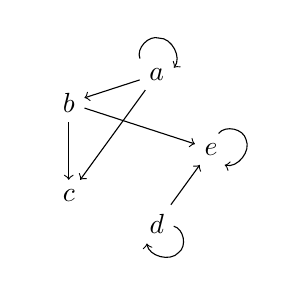
\begin{tikzpicture}
    %VARIABLES
    \pgfmathsetmacro{\gsize}{1}
    \pgfmathsetmacro{\gnum}{5}

    \foreach[count=\i] \element in {a,b,c,d,e} { %domain
        \node (\element) at (\i * 360 / \gnum:\gsize) {$\element$};
        \node (\element-) at (\i * 360 / \gnum:\gsize + 0.5) {};
      }
    \foreach \j/\l in {a/b, b/c, a/c, b/e, d/e} { %a to b
        \draw[->] (\j) -- (\l);
      }
    \foreach \j in {a,e,d} { %a to a
        \draw[->] (\j) to[bend left=65] (\j-)
        to[bend left=65] (\j);
      }
  \end{tikzpicture}
\end{center}
For Matrix Representation, this means that the matrix is anti-symmetric along the top left to bottom right diagonal:
\begin{center}
  $
    \bordermatrix{ & a & b & c & d \cr
      a & - & \bar{u} & \bar{v} & \bar{x} \cr
      b & u & - & \bar{w} & \bar{y} \cr
      c & v & w & - & \bar{z} \cr
      d & x & y & z & - \cr }
  $
  where
  \begin{tabular}{c}
    $u \in \{0,1\}$ \\
    $\vdots$        \\
    $z \in \{0,1\}$
  \end{tabular}
\end{center}

A binary relation of R on set $A$ is \textbf{Transitive} if for \textit{every} three elements $x,y,z \in A$,
if $x$R$y$ and $y$R$z$, then $x$R$z$. Logically, ($x$R$y \land y$R$z) \implies x$R$z$.
For Arrow Diagrams, this means the graph follows a hierarchy or kind of flow:
\begin{center}
  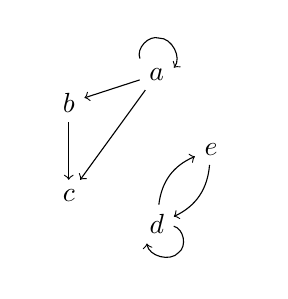
\begin{tikzpicture}
    %VARIABLES
    \pgfmathsetmacro{\gsize}{1}
    \pgfmathsetmacro{\gnum}{5}

    \foreach[count=\i] \element in {a,b,c,d,e} { %domain
        \node (\element) at (\i * 360 / \gnum:\gsize) {$\element$};
        \node (\element-) at (\i * 360 / \gnum:\gsize + 0.5) {};
      }
    \foreach \j/\l in {a/b,b/c,a/c} { %a to b
        \draw[->] (\j) -- (\l);
      }
    \foreach \j/\l in {d/e} { %a to b AND b to a
        \draw[->] (\j) to[bend left=20 / \gsize + 10] (\l);
        \draw[->] (\l) to[bend left=20 / \gsize + 10] (\j);
      }
    \foreach \j in {d,a} { %a to a
        \draw[->] (\j) to[bend left=65] (\j-)
        to[bend left=65] (\j);
      }
  \end{tikzpicture}
\end{center}
For Matrix Representation, it is much more difficult to determine transitivity, but here is an example:
\[
  \bordermatrix{ & a & b & c & d & e \cr
    a & 1 & 1 & 1 & 0 & 0 \cr
    b & 0 & 0 & 1 & 0 & 0 \cr
    c & 0 & 0 & 0 & 0 & 0 \cr
    d & 0 & 0 & 0 & 1 & 1 \cr
    e & 0 & 0 & 0 & 1 & 0 \cr }
\]

\subsection{Directed graphs, paths, and cycles}

A directed graph, or \textbf{Diagraph}, consists of a pair $(V,E)$, where $V$ is the set of vertices
and $E$ is the set of \textit{directed edges}. It is a subset of $V \times V$.
\begin{itemize}
  \item indegree: \# of edges pointing towards a vertex, $\text{indegree}(u) = \left\lvert\{v : (v,u) \in E\}\right\rvert$
  \item outdegree: \# of edges pointing away from a vertex, $\text{outdegree}(u) = \left\lvert\{u : (v,u) \in E\}\right\rvert$
\end{itemize}
A digraph is organized into a cartesian pair of the set of vertices and edge pairs:
\begin{align*}
  \text{Graph } G & = (V,E)                      \\
  V               & = \{a,b,c,d\}                \\
  E               & = \{(a,b),(b,c)(a,c),(d,d)\}
\end{align*}
\begin{center}
  \begin{tikzpicture}
    %VARIABLES
    \pgfmathsetmacro{\gsize}{1}
    \pgfmathsetmacro{\gnum}{4}

    \foreach[count=\i] \element in {a,b,c,d} { %domain
        \node (\element) at (\i * 360 / \gnum:\gsize) {$\element$};
        \node (\element-) at (\i * 360 / \gnum:\gsize + 0.5) {};
      }
    \foreach \j/\l in {a/b,b/c,a/c} { %a to b
        \draw[->] (\j) -- (\l);
      }
    \foreach \j/\l in {} { %a to b AND b to a
        \draw[->] (\j) to[bend left=20 / \gsize + 10] (\l);
        \draw[->] (\l) to[bend left=20 / \gsize + 10] (\j);
      }
    \foreach \j in {d} { %a to a
        \draw[->] (\j) to[bend left=65] (\j-)
        to[bend left=65] (\j);
      }
  \end{tikzpicture}
\end{center}
\begin{align*}
  \text{indegree}(c) & = 2 & \text{outdegree}(a) & = 2 & a & \text{ is the \underline{tail} of edge $(a,b)$} \\
  \text{indegree}(d) & = 1 & \text{outdegree}(d) & = 1 & b & \text{ is the \underline{head} of edge $(a,b)$} \\
\end{align*}

A digraph is mathematically the same as a relation. Here is an example of the internet as a graph:
\begin{align*}
  \text{Graph } G & = (V,E)                                                     \\
  V               & = \text{ set of all URLs}                                   \\
  E               & = \text{ set of all hyperlinks from one URL to another URL}
\end{align*}
\begin{align*}
  B   & = \text{ Blog}                   \\
  P   & = \text{ Pediatrician website}   \\
  PC  & = \text{ Pharmaceutical Company} \\
  AoP & = \text{ Academy of Pediatrics}
\end{align*}
\begin{center}
  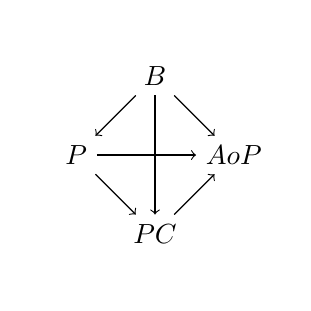
\begin{tikzpicture}
    %VARIABLES
    \pgfmathsetmacro{\gsize}{1}
    \pgfmathsetmacro{\gnum}{4}

    \foreach[count=\i] \element in {B, P, PC, AoP} { %domain
        \node (\element) at (\i * 360 / \gnum:\gsize) {$\element$};
        \node (\element-) at (\i * 360 / \gnum:\gsize + 0.5) {};
      }
    \foreach \j/\l in {B/P, B/PC, B/AoP, P/PC, P/AoP, PC/AoP} { %a to b
        \draw[->] (\j) -- (\l);
      }
    \foreach \j/\l in {} { %a to b AND b to a
        \draw[->] (\j) to[bend left=20 / \gsize + 10] (\l);
        \draw[->] (\l) to[bend left=20 / \gsize + 10] (\j);
      }
    \foreach \j in {} { %a to a
        \draw[->] (\j) to[bend left=65] (\j-)
        to[bend left=65] (\j);
      }
  \end{tikzpicture}
\end{center}

\subsubsection*{Walks in Directed Graphs}

\subsection{Composition of relations}
\subsection{Graph powers and the transitive closure}
\subsection{Matrix multiplication and graph powers}
\subsection{Partial orders}
\subsection{Strict orders and directed acyclic graphs}
\subsection{Equivalence relations}
\subsection{N-ary relations and relational databases}